\begin{figure*}[htb]
\setlength{\abovecaptionskip}{5pt plus 3pt minus 2pt}
\setlength{\belowcaptionskip}{-15pt plus 3pt minus 2pt}
\centering
% \includegraphics[width=\linewidth]{./images/Fight_results_with_circles.pdf}
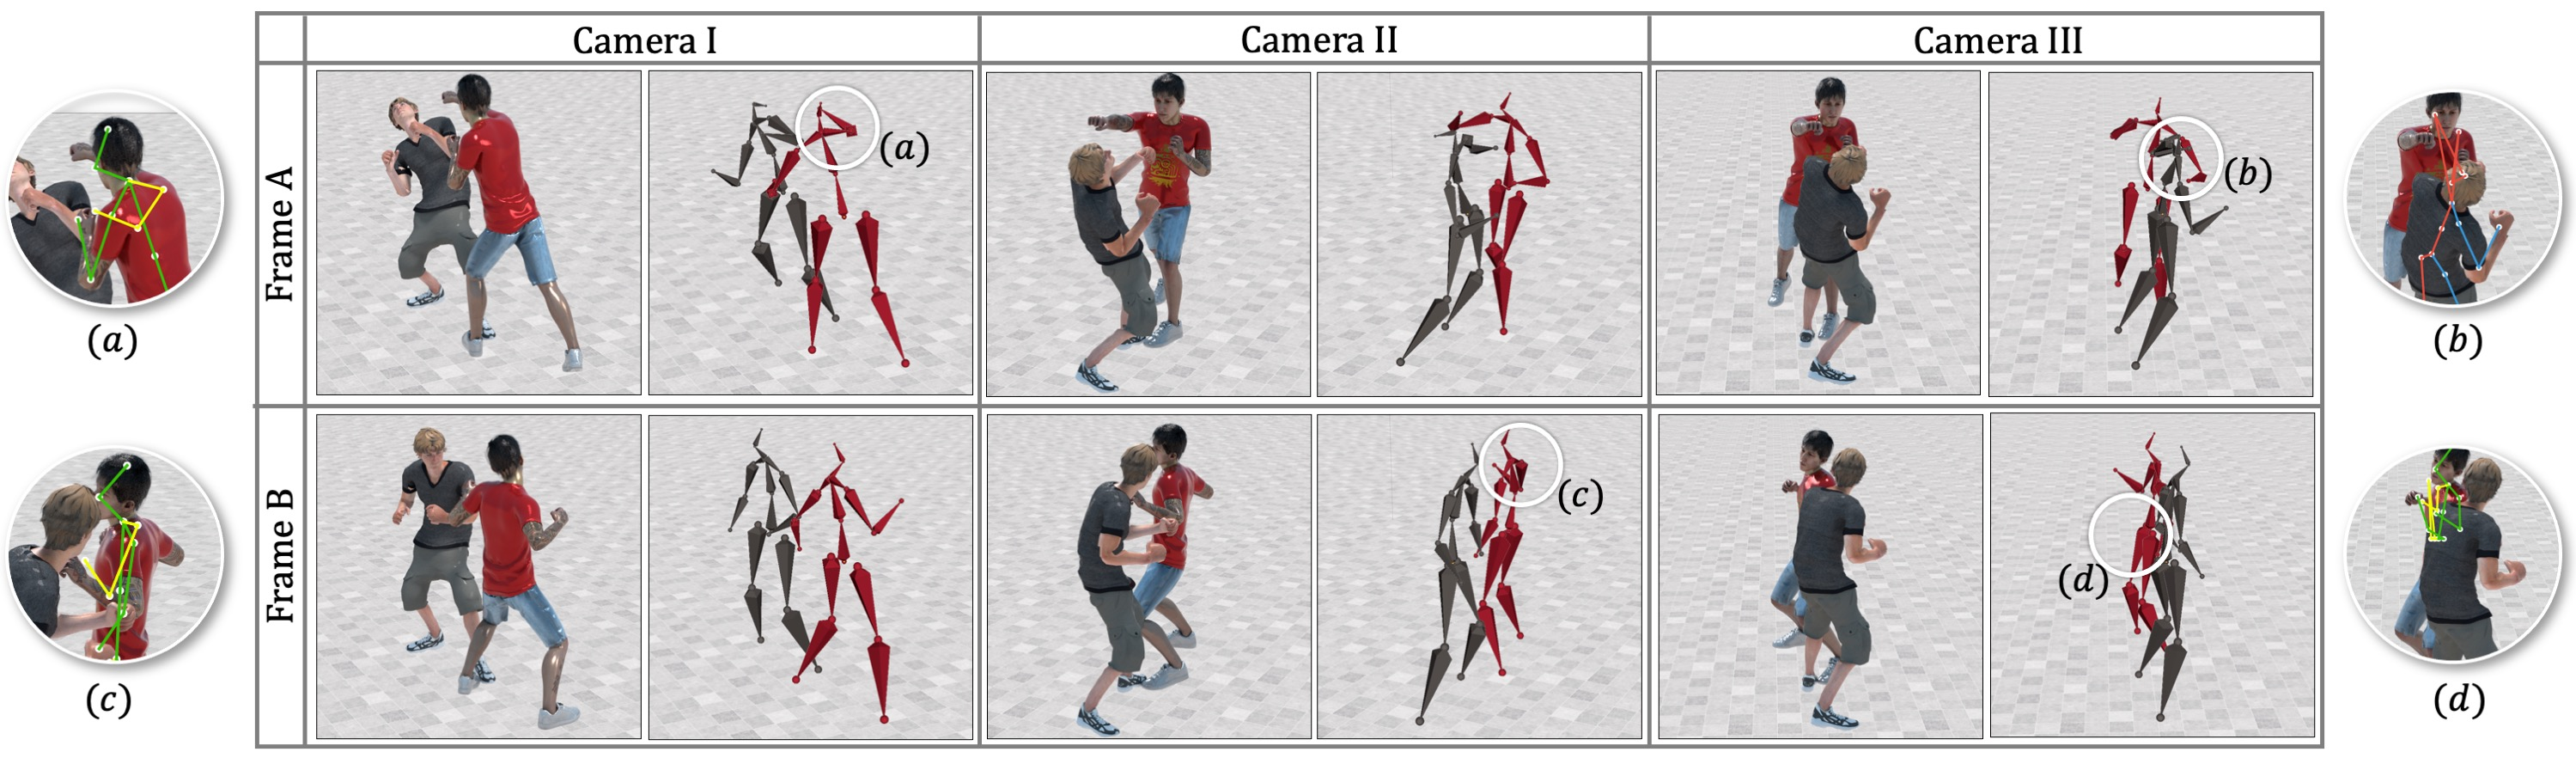
\includegraphics[width=\linewidth]{./images/Fight_results_with_circles_2_ROWS_new_design.jpg}
\caption{Results on multi-person synthetic videos.
% Our method reconstructs correct 3D motion although it takes inaccurate 2D joints for input. 
%Let \emph{gray fighter} and \emph{red fighter} denote the fighter wearing a gray and a red shirt, respectively. 
\sr{In the zoomed-in circular images we depict 2D pose estimations, which are erroneous due to occlusion. A matching circle in the center rectangular image shows that 
our method reconstructs correct 3D motion although it takes inaccurate 2D joints for input. 
% the motion reconstruction has not been affected by the erroneous 2D estimation.
}
%Several error examples are depicted in the zoomed-in circular insets: % (a) The right hand of the red fighter is self-occluded, so its 2D pose conveys a large error;
% (b) The nose tip of the gray fighter is erroneously detected next to the right eye of the red fighter, and his left arm is mismatched;
% (c) Erroneous 2D pose estimation of the red fighter's right hand;
% (d) The red fighter is mostly occluded; hence the 2D joint estimation of his body is a 
% blunder. 
} 
\label{fig:fight_results_with_circles}
\end{figure*}